\chapter{Homogeneous parallel ensembles: Bagging and random forests\label{Ch02}}
\section{Bagging: Bootstrap aggregating}
\textbf{Bagging}, short for \textbf{bootstrap aggregating}, was introduced by Leo Breiman in 1996. The
name refers to how bagging achieves ensemble diversity (through bootstrap sampling) and performs ensemble prediction (through model aggregating).
\begin{figure}
    \centering
    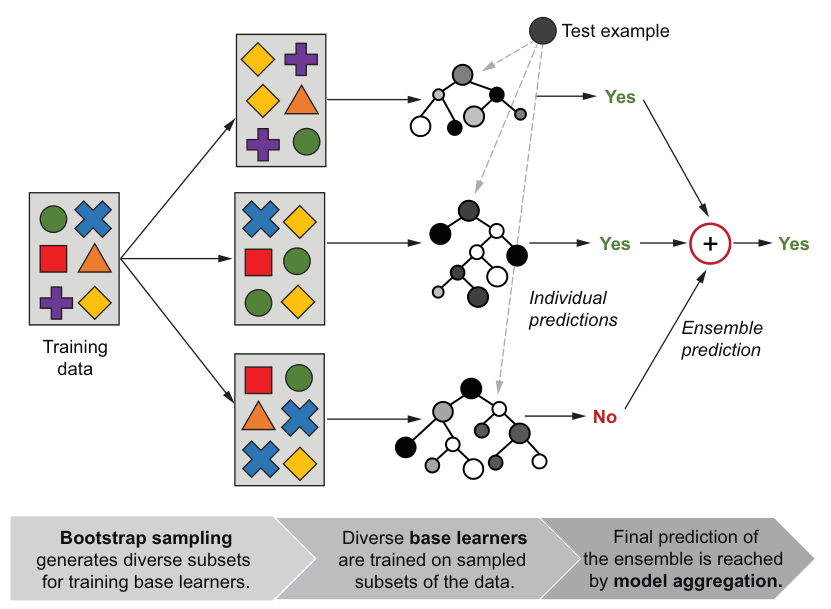
\includegraphics{../Figures/fig2-2.png}
    \caption{Bagging, illustrated. Bagging uses bootstrap sampling to generate similar but not exactly identical subsets (observe the replicates here) from a single data set. Models are trained on each of these subsets, resulting in similar but not exactly identical base estimators. Given a test example, the individual base-estimator predictions are aggregated into a final ensemble prediction. Also observe that training examples may repeat in the replicated subsets; this is a consequence of bootstrap sampling.}
\end{figure}

\figures{fig2-3}{
    Bootstrap sampling illustrated on a data set of six examples. By sampling with
    replacement, we can get a bootstrap sample size of six, containing only four unique objects
    but with repeats. Performing bootstrap sampling several times produces several replicates
    of the original data set—all of them with repeats.
}

\section{Random forests}
Random forests use a modified tree learning algorithm, which first randomly samples features before creating a decision node. The resulting tree is a \textbf{randomized decision tree}, which is a new type of base estimator.

Thus, random forests contain two types of randomization: (1) bootstrap sampling, similar to bagging; and (2) random feature sampling for learning randomized decision trees.

\figures{fig2-7}{Random forests use a modified tree learning algorithm, where a random feature subset is
    first chosen before the best splitting criterion for each decision node is identified. The unshaded columns
    represent features that have been left out; the lightly shaded columns represent available features from
    which the best feature is chosen, shown in the darkly shaded columns.}
\subsection*{Feature importances}
One benefit of using random forests is that they also provide a natural mechanism for scoring features based on their importance. This means that we can rank features to identify the most important ones and drop less effective features, thus performing feature selection!

\section{More homogeneous parallel ensembles}
We’ve seen two important parallel homogeneous ensemble methods: bagging and
random forests. Let’s now explore a few variants that were developed for large data
sets (e.g., recommendation systems) or high-dimensional data (e.g., image or text
databases). These include bagging variants such as pasting, random subspaces and
random patches, and an extreme random forest variant called Extra Trees. All these
methods introduce randomization in different ways to ensure ensemble diversity.
\subsection*{Pasting}
Bagging uses bootstrap sampling, or sampling with replacement. If, instead, we sample subsets for training \textbf{without replacement}, we have a variant of bagging known as \textbf{pasting}. \important{Pasting was designed for very large data sets, where sampling with replacement isn’t necessary}. Instead, because training full models on data sets of such scale is difficult, pasting aims to take small pieces of the data by sampling without replacement.
\begin{tcolorbox}[title=TIP]
    BaggingClassifier can easily be extended to perform pasting by setting bootstrap=False and making it subsample small subsets for training
    by setting max\_samples to a small fraction, say max\_samples=0.05.
\end{tcolorbox}